\documentclass{article}

\usepackage[preprint]{corl_2026}

\usepackage[utf8]{inputenc}
\usepackage[T1]{fontenc}
\usepackage{amsmath,amssymb,bm}
\usepackage{booktabs}
\usepackage{tabularx}
\usepackage{graphicx}
\usepackage[table]{xcolor}
\usepackage{tikz}
\usetikzlibrary{arrows.meta,positioning,calc,fit,backgrounds,decorations.pathmorphing}
\usepackage{pgfplots}
\pgfplotsset{compat=1.18}
\usepackage{listings}
\usepackage{microtype}
\usepackage{float}
\usepackage{caption}
\captionsetup{labelsep=period}

% ---------- notation and helpers shared by both layouts ----------
\newcommand{\code}[1]{\texttt{#1}}
\newcommand{\subl}[1]{{\scriptsize\color{black!60}#1}}
\definecolor{series1}{HTML}{2A78D6}
\definecolor{series2}{HTML}{EB6834}
\definecolor{band}{HTML}{E7EEF1}
\definecolor{codebg}{HTML}{F4F5F4}
\definecolor{stagefill}{HTML}{DFEAEF}
\definecolor{stageline}{HTML}{1F6F8B}
\lstset{
  language=Python,
  commentstyle=\color{black!55}\itshape,
  keywordstyle=\bfseries,
  stringstyle=\color{black!70},
  backgroundcolor=\color{codebg},
  frame=single, framerule=0pt, framesep=3pt,
  columns=fullflexible, keepspaces=true,
  breaklines=true, breakatwhitespace=false, showstringspaces=false,
  numbers=left, numberstyle=\tiny\color{black!45}\ttfamily, numbersep=5pt, stepnumber=1,
  xleftmargin=18pt, xrightmargin=2pt,
  aboveskip=1pt, belowskip=0pt,
  literate={ö}{{\"o}}1 {ä}{{\"a}}1 {·}{{$\cdot$}}1 {—}{{--}}1 {→}{{$\to$}}1,
}
% file header above a listing: path on the left, line range on the right
\newcommand{\snippethead}[2]{\par\noindent{\scriptsize\sffamily\color{black!60}\path{#1}\hfill\mbox{#2}}\par\nopagebreak\vspace{-2pt}}
\newcommand{\snippetelide}{\par\nopagebreak\vspace{-5pt}\noindent{\scriptsize\color{black!45}\ttfamily\hspace{6pt}$\vdots$}\par\nopagebreak\vspace{-6pt}}
\tikzset{
  blk/.style={draw=black!55, rounded corners=2pt, minimum height=8mm, align=center, font=\small, inner sep=3pt, fill=black!4},
  stage/.style={blk, fill=stagefill, draw=stageline, line width=0.8pt},
  sub/.style={font=\scriptsize\color{black!60}},
  arr/.style={-{Latex[length=2mm]}, thick, black!70},
  darr/.style={-{Latex[length=2mm]}, thick, dashed, black!55},
}
% a snippet (header + listing, possibly with elisions). The optional argument is the number of text lines that
% must still fit on the page before the snippet may start, so the header always stays with the first code lines;
% a long listing may then break across pages instead of leaving a large gap at the page bottom.
\newenvironment{snippetbox}[1][8]{\par\addvspace{4pt}\penalty0
  \ifdim\pagegoal=\maxdimen\else
    \ifdim\dimexpr\pagegoal-\pagetotal\relax<#1\baselineskip \newpage\fi
  \fi
  \lstset{aboveskip=1pt, belowskip=0pt}}{\par\addvspace{4pt}}

\lstset{basicstyle=\ttfamily\scriptsize}
\definecolor{seriesfix}{HTML}{2E8455}
\definecolor{seriesbad}{HTML}{9B3C8E}
\definecolor{series1}{HTML}{2F6DB5}
\definecolor{series2}{HTML}{C4581B}

% figure and table wrappers: placed exactly where they are referenced (no floating)
\newenvironment{myfigure}{\begin{figure}[H]\centering}{\end{figure}}
\newenvironment{mytable}{\begin{table}[H]\centering}{\end{table}}
\newcommand{\myfigcaption}[2]{\caption{#2}\label{#1}}
\newcommand{\mytabcaption}[2]{\caption{#2}\label{#1}}

\title{Two Arms, One Controller\\[2pt] \large Why the G1-D Hand Moves Faster than the UR5e Hand}

\author{
  Tri Wahyu Guntara\\
  Controller notes on the UWLab OmniReset code base\\
}

\raggedbottom

\begin{document}
\maketitle

%==============================================================================
\section{What the Policy Commands}
\label{sec:command}

Every tenth of a second the OmniReset policy~\cite{omnireset2026} writes six numbers. The first three ask the hand to move along the $x$, $y$ and $z$ axes of the robot base, and the last three ask it to turn about those same axes. The policy never names a joint angle or a torque. It names a small change of the hand pose, and a controller underneath turns that wish into motor torques.

The six numbers first pass through a scale. Both robots use the same one, 20 millimetres per unit for each translation and 0.2 radians per unit for the turn about $z$. The controller then builds a target pose by adding the scaled change to the pose the hand has \emph{right now},
\begin{equation}
\bm{x}_{\text{target}} = \bm{x}_{\text{measured}} + \bm{s} \odot \bm{a},
\end{equation}
where $\bm{a}$ is the policy output and $\bm{s}$ is the scale. Two details matter for the rest of this note. The target is rebuilt from the measured pose at every policy step, so the controller only ever chases a point one action ahead of the hand. And nothing limits the size of $\bm{a}$. A policy that outputs 5 asks for 100 millimetres just as easily as one that outputs 1 asks for 20.

Between two policy steps the physics engine advances twelve times, at 120 hertz. At each of those twelve substeps the controller measures the arm again and recomputes the torques, while the target stays fixed. Figure~\ref{fig:loop} shows the loop.

\begin{myfigure}
\resizebox{\linewidth}{!}{%
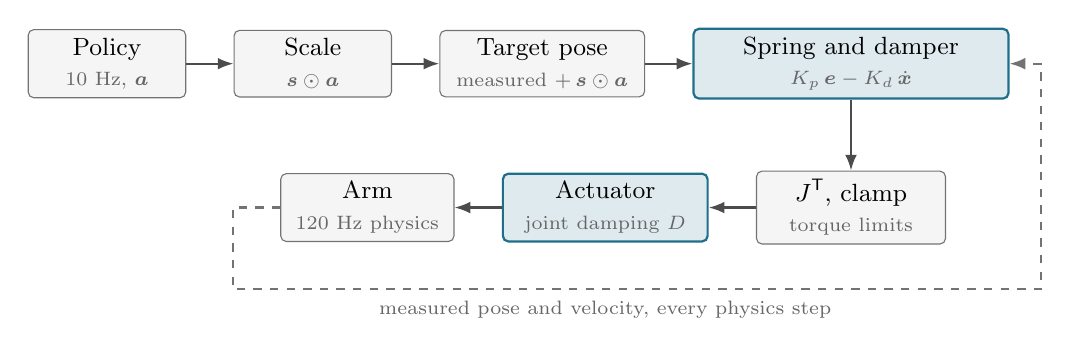
\begin{tikzpicture}[node distance=5mm and 6mm]
\node[blk, minimum width=20mm] (pol) {Policy\\\subl{10 Hz, $\bm a$}};
\node[blk, minimum width=20mm, right=of pol] (sc) {Scale\\\subl{$\bm s\odot\bm a$}};
\node[blk, minimum width=26mm, right=of sc] (tg) {Target pose\\\subl{measured $+\,\bm s\odot\bm a$}};
\node[stage, minimum width=40mm, right=of tg] (pd) {Spring and damper\\\subl{$K_p\,\bm e - K_d\,\dot{\bm x}$}};
\node[blk, minimum width=24mm, below=9mm of pd] (jt) {$J^{\mathsf T}$, clamp\\\subl{torque limits}};
\node[stage, minimum width=26mm, left=of jt] (act) {Actuator\\\subl{joint damping $D$}};
\node[blk, minimum width=22mm, left=of act] (arm) {Arm\\\subl{120 Hz physics}};
\draw[arr] (pol) -- (sc); \draw[arr] (sc) -- (tg); \draw[arr] (tg) -- (pd);
\draw[arr] (pd) -- (jt); \draw[arr] (jt) -- (act); \draw[arr] (act) -- (arm);
\draw[darr] (arm.west) -- ++(-6mm,0) |- ($(arm.south)+(0,-6mm)$) -| ($(pd.east)+(4mm,0)$) -- (pd.east);
\node[sub] at ($(act.south)+(0,-8.5mm)$) {measured pose and velocity, every physics step};
\end{tikzpicture}}
\myfigcaption{fig:loop}{The controller of both robots. The policy runs at 10 hertz and everything inside the loop runs at 120 hertz. The two outlined blocks hold the settings in which the robots differ.}
\end{myfigure}

%==============================================================================
\section{A Spring, a Damper and a Jacobian}
\label{sec:law}

The controller behaves like an invisible spring stretched between the hand and the target, with a shock absorber mounted beside it~\cite{khatib1987unified}. The spring pulls the hand toward the target with a force that grows with the distance. The shock absorber, which engineers call a damper, pushes against the hand with a force that grows with its speed. For the force $\bm F$ on the hand the law reads
\begin{equation}
\bm F = K_p\,\bm e - K_d\,\dot{\bm x},
\end{equation}
where $\bm e$ is the pose error, the gap between target and hand, and $\dot{\bm x}$ is the hand velocity. The stiffness $K_p$ sets how hard the spring pulls, and the damping $K_d$ sets how hard the shock absorber resists motion.

A force at the hand is not something a motor can produce directly. The Jacobian $J$, a matrix that relates joint speeds to hand speed, translates the force into one torque per joint. The controller also adds a small posture term for the seven-jointed G1-D, which keeps the elbow near a preferred angle without moving the hand, and the actuator adds its own joint damping $D$. The full torque on the joints is therefore
\begin{equation}
\bm\tau = J^{\mathsf T}\big(K_p\,\bm e - K_d\,J\dot{\bm q}\big) + \bm\tau_{\text{posture}} - D\,\dot{\bm q},
\end{equation}
where $\dot{\bm q}$ collects the joint speeds. The torques are then clipped to each motor's limit. Notice what the law leaves out. It never accounts for how heavy the arm is. A heavy arm and a light arm receive the same force for the same error, and they respond very differently to it. That omission is the root of this whole story.

The configuration files do not store $K_d$ directly. They store a number called the damping ratio, written $\zeta$, and convert it with the rule
\begin{equation}
K_d = 2\,\zeta\sqrt{K_p}.
\end{equation}
This rule is exact only for a hand that weighs one kilogram. Section~\ref{sec:mass} shows what it means for real arms, and Figure~\ref{fig:springs} pictures the two hands as masses on springs.

\begin{myfigure}
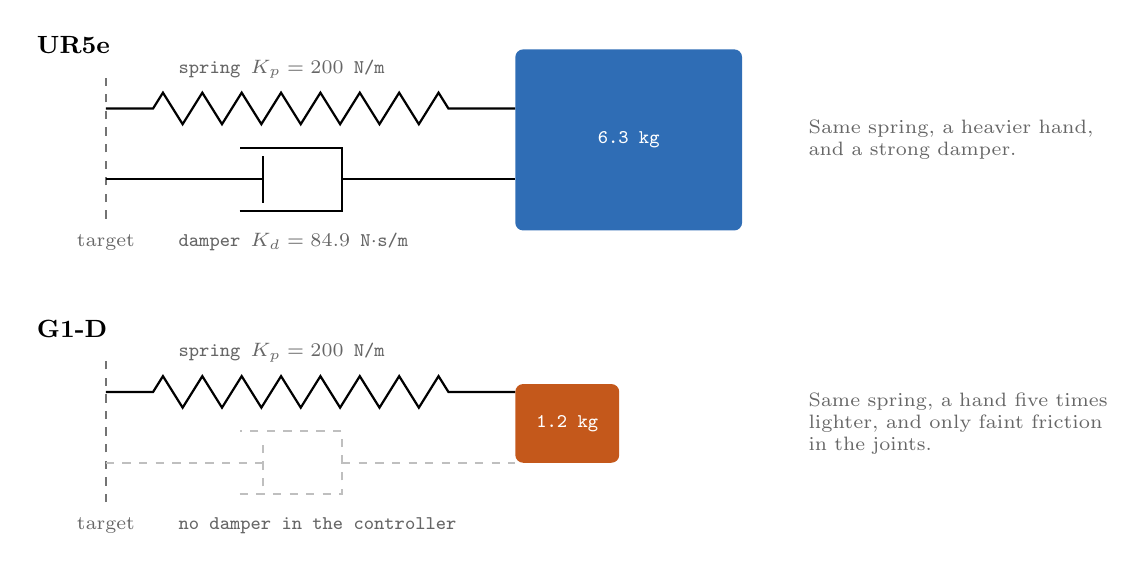
\begin{tikzpicture}[x=1mm,y=1mm,
  spring/.style={decorate, decoration={zigzag, segment length=5mm, amplitude=2mm, pre length=6mm, post length=6mm}, thick}]
\foreach \row/\y/\name/\mass/\w/\col/\damp/\note in {0/0/UR5e/6.3 kg/24/series1/1/{Same spring, a heavier hand, and a strong damper.}, 1/-36/G1-D/1.2 kg/11/series2/0/{Same spring, a hand five times lighter, and only faint friction in the joints.}}{
  \node[font=\small\bfseries, anchor=west] at (0,\y+12) {\name};
  \draw[thick, dashed, black!55] (10,\y-10) -- (10,\y+8);
  \node[font=\scriptsize, black!60] at (10,\y-13) {target};
  \draw[spring] (10,\y+4) -- (62,\y+4);
  \node[font=\scriptsize\ttfamily, black!60, anchor=west] at (18,\y+9) {spring $K_p = 200$ N/m};
  \ifnum\damp=1
    \draw[thick] (10,\y-5) -- (30,\y-5) (30,\y-8) -- (30,\y-2) (27,\y-9) -- (40,\y-9) -- (40,\y-1) -- (27,\y-1) (40,\y-5) -- (62,\y-5);
    \node[font=\scriptsize\ttfamily, black!60, anchor=west] at (18,\y-13) {damper $K_d = 84.9$ N$\cdot$s/m};
  \else
    \draw[thick, black!25, dashed] (10,\y-5) -- (30,\y-5) (30,\y-8) -- (30,\y-2) (27,\y-9) -- (40,\y-9) -- (40,\y-1) -- (27,\y-1) (40,\y-5) -- (62,\y-5);
    \node[font=\scriptsize\ttfamily, black!60, anchor=west] at (18,\y-13) {no damper in the controller};
  \fi
  \fill[\col, rounded corners=1mm] (62,\y-\w/2+0.5) rectangle (62+1.2*\w,\y+\w/2-0.5);
  \node[font=\scriptsize\ttfamily, white] at (62+0.6*\w,\y) {\mass};
  \node[font=\scriptsize, black!60, anchor=west, text width=38mm] at (98,\y) {\note};
}
\end{tikzpicture}
\myfigcaption{fig:springs}{The two hands seen as masses on springs, moving sideways along $y$ in the test pose of Section~\ref{sec:measure}. The masses are the effective task-space inertia measured from the simulator.}
\end{myfigure}

%==============================================================================
\section{Where the Two Robots Differ}
\label{sec:differ}

The G1-D configuration was written to mirror the UR5e recipe, and most of its numbers are indeed identical. Table~\ref{tab:settings} lists every setting that reaches the controller or the actuator, with the rows that differ shaded.

\begin{mytable}
\small
\begin{tabular}{@{}p{0.36\linewidth}p{0.29\linewidth}p{0.29\linewidth}@{}}
\toprule
Setting & UR5e & G1-D with Dex1 \\
\midrule
Arm joints under control & 6 & 7 \\
Action scale per unit & 20 mm, 0.2 rad about $z$ & 20 mm, 0.2 rad about $z$ \\
Stiffness $K_p$, translation and rotation & 200 N/m, 3 N$\cdot$m/rad & 200 N/m, 3 N$\cdot$m/rad \\
\rowcolor{band} Damping ratio $\zeta$, translation and rotation & 3 and 1 & 0 and 0 \\
\rowcolor{band} Controller damping $K_d$ & 84.9 N$\cdot$s/m, 3.46 N$\cdot$m$\cdot$s/rad & none \\
\rowcolor{band} Actuator joint damping $D$ & none & 1 N$\cdot$m$\cdot$s/rad on every joint \\
\rowcolor{band} Posture task in the null space & none & stiffness 2, damping 2.83 \\
\rowcolor{band} Torque limits & 150 N$\cdot$m shoulder and elbow, 28 N$\cdot$m wrist & 25 N$\cdot$m, 5 N$\cdot$m wrist pitch and yaw \\
\rowcolor{band} Joint speed limits & 1.57 rad/s large joints, 3.14 rad/s wrist & 37 rad/s, 22 rad/s wrist \\
\rowcolor{band} Effective hand mass along $y$ at the test pose & 6.3 kg & 1.2 kg \\
\rowcolor{band} Inertia of the last wrist joint & 0.0167 kg$\cdot$m$^2$ & 0.0041 kg$\cdot$m$^2$ \\
Physics rate and policy rate & 120 Hz and 10 Hz & 120 Hz and 10 Hz \\
Action clipping & none & none \\
\bottomrule
\end{tabular}
\mytabcaption{tab:settings}{Controller and actuator settings of the two robots in the stage 1 training configuration.}
\end{mytable}

Three differences dominate. The G1-D controller has no damper at all, the G1-D hand is about five times lighter, and its joint speed limits are so high that they never come into play. The UR5e speed limit of 1.57 radians per second, on the other hand, quietly caps how fast its large joints can swing.

The settings come straight from three places in the code. The UR5e action is defined as follows.

\begin{snippetbox}[10]
\snippethead{source/uwlab_tasks/uwlab_tasks/manager_based/manipulation/omnireset/config/ur5e_robotiq_2f85/actions.py}{lines 15 to 23}
\begin{lstlisting}[firstnumber=15]
UR5E_ROBOTIQ_2F85_RELATIVE_OSC = RelCartesianOSCActionCfg(
    asset_name="robot",
    joint_names=["shoulder.*", "elbow.*", "wrist.*"],
    body_name="wrist_3_link",
    scale_xyz_axisangle=(0.02, 0.02, 0.02, 0.02, 0.02, 0.2),
    motion_stiffness=(200.0, 200.0, 200.0, 3.0, 3.0, 3.0),
    motion_damping_ratio=(3.0, 3.0, 3.0, 1.0, 1.0, 1.0),
    torque_limit=(150.0, 150.0, 150.0, 28.0, 28.0, 28.0),
)
\end{lstlisting}
\end{snippetbox}

The G1-D action copies the stiffness and the scale but sets every damping ratio to zero, and its comment records why.

\begin{snippetbox}[10]
\snippethead{source/uwlab_tasks/uwlab_tasks/manager_based/manipulation/omnireset/config/g1d_dex1/actions.py}{lines 27 to 42}
\begin{lstlisting}[firstnumber=27]
G1D_DEX1_RELATIVE_OSC = RelCartesianOSCActionCfg(
    asset_name="robot",
    joint_names=G1D_ARM_JOINT_NAMES,
    body_name=G1D_EE_BODY_NAME,
    scale_xyz_axisangle=(0.02, 0.02, 0.02, 0.02, 0.02, 0.2),
    motion_stiffness=(200.0, 200.0, 200.0, 3.0, 3.0, 3.0),
    # No explicit task-space damping: it is unstable on the light G1-D wrist links; the damping is provided
    # implicitly by the arm actuator (see IMPLICIT_G1D_DEX1 in uwlab_assets).
    motion_damping_ratio=(0.0, 0.0, 0.0, 0.0, 0.0, 0.0),
    torque_limit=G1D_TORQUE_LIMIT,
    jacobian_fn=G1D_JACOBIAN_FN,
    # 7-DoF arm: hold the default elbow configuration in the null space of the task
    nullspace_stiffness=2.0,
    nullspace_damping_ratio=1.0,
    nullspace_joint_pos=G1D_DEFAULT_ARM_JOINT_POS,
)
\end{lstlisting}
\end{snippetbox}

The damping that the G1-D does have lives in its arm actuator, one newton metre per radian per second on each joint.

\begin{snippetbox}[10]
\snippethead{source/uwlab_assets/uwlab_assets/robots/unitree_g1d_dex1/g1d_dex1.py}{lines 136 to 150}
\begin{lstlisting}[firstnumber=136]
IMPLICIT_G1D_DEX1.actuators = {
    "arm": ImplicitActuatorCfg(
        joint_names_expr=G1D_ARM_JOINT_REGEX,
        stiffness=0.0,
        # Joint damping lives here (PhysX applies it implicitly, stable at any gain) instead of in the OSC: the
        # wrist links weigh ~85 g (I ~ 5e-4 kg m^2 about the roll axis), and an explicit task-space damping torque
        # of a few N m s/rad at 120 Hz overshoots the velocity each substep and diverges within a handful of
        # substeps (verified with scripts_v2/tools/debug_reset_env-style probes on 2026-10-26). The UR5e gets away
        # with explicit damping only because its wrist links are ~10x heavier.
        damping=1.0,
        effort_limit_sim=G1D_EFFORT_LIMITS,
        velocity_limit_sim=G1D_VELOCITY_LIMITS,
    ),
    "gripper": DEX1_GRIPPER_ACTUATOR,
}
\end{lstlisting}
\end{snippetbox}

The inertia figures in Table~\ref{tab:settings} come from the simulator itself. The effective hand mass is the task-space inertia, a quantity that Section~\ref{sec:mass} introduces, evaluated at the default arm pose of each robot.

%==============================================================================
\section{One Mass on a Spring}
\label{sec:mass}

A whole arm is complicated, but along any single direction it behaves much like one mass. That mass is called the task-space inertia and is written $\Lambda$. It answers a simple question. If you push the hand with one newton, how quickly does it start to move? Physics gives the answer through the joint inertia matrix $M$ and the Jacobian,
\begin{equation}
\Lambda = \big(J M^{-1} J^{\mathsf T}\big)^{-1}.
\end{equation}
With that single mass in hand, the controller reduces to the textbook mass on a spring with a damper,
\begin{equation}
\Lambda\,\ddot x = K_p\,(x_{\text{target}} - x) - K_d\,\dot x .
\end{equation}
Two numbers describe how such a system moves. The natural frequency tells how quickly it reacts, and the true damping ratio tells whether it overshoots,
\begin{equation}
\omega_n = \sqrt{\frac{K_p}{\Lambda}}, \qquad \zeta_{\text{true}} = \frac{K_d}{2\sqrt{K_p\,\Lambda}} .
\end{equation}
For the UR5e moving along $y$, with a mass of 6.3 kilograms, the natural frequency is 5.6 radians per second and the true damping ratio is 1.2. The setting of 3 in the configuration file therefore produces a hand that is a little more than critically damped, which is exactly the calm, no-overshoot motion the UR5e shows. For the G1-D, with a mass of 1.2 kilograms, the same spring gives a natural frequency of 13 radians per second, more than twice as fast, and the controller adds no damping at all.

\paragraph{The speed the hand settles at.} Because the target is rebuilt from the measured pose at every policy step, a policy that holds the same action keeps the spring stretched by the same amount, step after step. The hand then stops accelerating once the damper pushes back as hard as the spring pulls. Setting the two forces equal gives the cruising speed,
\begin{equation}
v_{\text{cruise}} = \frac{K_p\, s\, a}{K_d}.
\label{eq:cruise}
\end{equation}
For the UR5e with an action of one, this is 200 times 0.02 divided by 84.9, or 47 millimetres per second. Notice that the hand mass has dropped out. Once the damper is present, the cruising speed depends only on the gains, the scale and the action. Without a damper the formula breaks down, and the only thing left to stop the G1-D hand is the faint joint damping in its actuator. The cruising speed also grows in direct proportion to the action $a$. Keep this in mind for Section~\ref{sec:policy}, because the policy is free to choose $a$.

%==============================================================================
\section{Measuring the Two Arms}
\label{sec:measure}

Theory is only half of the argument, so both arms were tested in simulation with the training configuration. Each arm started from its default pose with gravity off, as in training. The test then gave one action of plus one for a single policy step, waited, held the same action for one full second, and finally released it. The hand was recorded at every physics step. Figure~\ref{fig:stepy} shows the sideways motion.

\begin{myfigure}
\begin{tikzpicture}
\begin{axis}[width=\linewidth, height=0.42\linewidth, xmin=0, xmax=4, ymin=-15, ymax=440, ytick={0,100,200,300,400},
  xlabel={time (s)}, ylabel={hand displacement along $y$ (mm)}, label style={font=\small}, tick label style={font=\footnotesize},
  grid=major, grid style={black!10}, axis lines*=left, clip mode=individual,
  legend style={font=\footnotesize, draw=none, at={(0.5,-0.24)}, anchor=north, legend columns=2, /tikz/every even column/.append style={column sep=4mm}}]
  \fill[band] (axis cs:1.0,-15) rectangle (axis cs:1.1,440);
  \fill[band] (axis cs:2.0,-15) rectangle (axis cs:3.0,440);
  \node[font=\scriptsize, black!60, anchor=south] at (axis cs:1.05,440) {one step};
  \node[font=\scriptsize, black!60, anchor=south] at (axis cs:2.5,440) {command held for 1 s};
  \addplot[series1, thick] table[x=t, y=ur] {step_y.dat}; \addlegendentry{UR5e, as trained}
  \addplot[series1, thick, dashed] table[x=t, y=urnod] {step_y.dat}; \addlegendentry{UR5e with its damper removed}
  \addplot[series2, thick] table[x=t, y=g1] {step_y.dat}; \addlegendentry{G1-D, as trained}
  \addplot[seriesfix, thick] table[x=t, y=fix] {step_y.dat}; \addlegendentry{G1-D with translational damping}
\end{axis}
\end{tikzpicture}
\myfigcaption{fig:stepy}{Sideways motion of the hand along $y$. The shaded bands mark when the command was active. With its damper, the UR5e hand cruises at 43 millimetres per second, close to the 47 that Equation~\eqref{eq:cruise} predicts. The G1-D hand reaches 224 millimetres per second, five times faster. Remove the damper from the UR5e and it runs even faster, then keeps sliding for 17 centimetres after the command ends. Give the G1-D the UR5e translational damping and it falls in line with the UR5e.}
\end{myfigure}

The figure carries the central result. The difference in speed comes almost entirely from the missing damper. The UR5e without its damper runs even faster than the G1-D, because nothing but its joint speed limits stand in its way. The G1-D at least has its faint joint damping, which is also why it stops quickly after the command ends rather than coasting. Table~\ref{tab:speeds} collects all six directions.

\begin{mytable}
\small
\begin{tabularx}{\linewidth}{@{}l*{4}{>{\raggedleft\arraybackslash}X}@{}}
\toprule
Direction & UR5e as trained & G1-D as trained & G1-D, translational damping & UR5e, no damper \\
\midrule
$x$, peak speed & 43 mm/s & 24 mm/s & 13 mm/s & 226 mm/s \\
$y$, peak speed & 43 mm/s & 224 mm/s & 42 mm/s & 321 mm/s \\
$z$, peak speed & 43 mm/s & 240 mm/s & 42 mm/s & 330 mm/s \\
Turn about $x$, peak rate & 1.0 $^\circ$/s & 8.4 $^\circ$/s & 8.1 $^\circ$/s & 24 $^\circ$/s \\
Turn about $y$, peak rate & 1.0 $^\circ$/s & 5.5 $^\circ$/s & 3.2 $^\circ$/s & 19 $^\circ$/s \\
Turn about $z$, peak rate & 17 $^\circ$/s & 34 $^\circ$/s & 22 $^\circ$/s & unstable \\
\bottomrule
\end{tabularx}
\mytabcaption{tab:speeds}{Peak hand speed while an action of one is held for one second, measured at the default arm pose.}
\end{mytable}

The G1-D $x$ direction is the exception. In the default pose, moving the hand forward along $x$ appears to need large joint speeds, so even the faint joint damping slows it a great deal. The large effective mass in that direction, about 8 kilograms, points the same way. Real episodes visit many poses, so this direction is not always slow. Every number here belongs to one pose and would change somewhat in another.

Rotation tells a similar story. The G1-D turns two to eight times faster than the UR5e, and the translational damper alone barely changes that. Figure~\ref{fig:steprz} shows the turn about $z$ and introduces the problem that the next section explains.

\begin{myfigure}
\begin{tikzpicture}
\begin{axis}[width=\linewidth, height=0.42\linewidth, xmin=0, xmax=4, ymin=-12, ymax=40, ytick={-10,0,10,20,30,40},
  xlabel={time (s)}, ylabel={hand rotation about $z$ (degrees)}, label style={font=\small}, tick label style={font=\footnotesize},
  grid=major, grid style={black!10}, axis lines*=left, clip mode=individual,
  legend style={font=\footnotesize, draw=none, at={(0.5,-0.24)}, anchor=north, legend columns=2, /tikz/every even column/.append style={column sep=4mm}}]
  \fill[band] (axis cs:1.0,-12) rectangle (axis cs:1.1,40);
  \fill[band] (axis cs:2.0,-12) rectangle (axis cs:3.0,40);
  \node[font=\scriptsize, black!60, anchor=south] at (axis cs:1.05,40) {one step};
  \node[font=\scriptsize, black!60, anchor=south] at (axis cs:2.5,40) {command held for 1 s};
  \addplot[series1, thick] table[x=t, y=ur] {step_rz.dat}; \addlegendentry{UR5e, as trained}
  \addplot[series2, thick] table[x=t, y=g1] {step_rz.dat}; \addlegendentry{G1-D, as trained}
  \addplot[seriesbad, thin] table[x=t, y=rot] {step_rz.dat}; \addlegendentry{G1-D, rotational damping in the controller}
  \addplot[seriesfix, thick] table[x=t, y=fix] {step_rz.dat}; \addlegendentry{G1-D, translational and wrist damping 2}
\end{axis}
\end{tikzpicture}
\myfigcaption{fig:steprz}{Rotation of the hand about $z$. Adding rotational damping inside the controller, as the UR5e does, makes the G1-D wrist chatter violently, and the commanded turn is lost in the shaking. The chatter begins at rest, before any command arrives, which shows that the damping itself drives it. Adding the damping to the wrist joints in the actuator instead slows the turn to 14 degrees per second, close to the UR5e, with no chatter.}
\end{myfigure}

%==============================================================================
\section{Why the G1-D Lost Its Damper}
\label{sec:stability}

The missing damper was a deliberate choice. The comment in the G1-D action configuration records that explicit damping in the controller made the light wrist unstable. Figure~\ref{fig:steprz} confirms that warning, and a short calculation explains it.

The controller computes its damping torque from the velocity it measured at the start of a physics step, then holds that torque for the whole step of $\Delta t = 1/120$ of a second. Consider a single joint with inertia $I$ spinning at speed $v$. After one step the damping torque has changed the speed to
\begin{equation}
v_{k+1} = \Big(1 - \frac{K_d\,\Delta t}{I}\Big)\, v_k .
\end{equation}
If the bracket lies between minus one and one, the speed shrinks every step and the joint settles. If the damping is too strong for the inertia, the bracket drops below minus one, and the joint reverses direction faster than it was moving before. Each step then makes the motion larger. The stability condition is therefore
\begin{equation}
\frac{K_d\,\Delta t}{I} < 2 .
\end{equation}
The rotational damping of the UR5e recipe, 3.46 newton metres per radian per second, acts almost directly on the last wrist joint. Figure~\ref{fig:stab} compares the ratio for each wrist joint of the two robots.

\begin{myfigure}
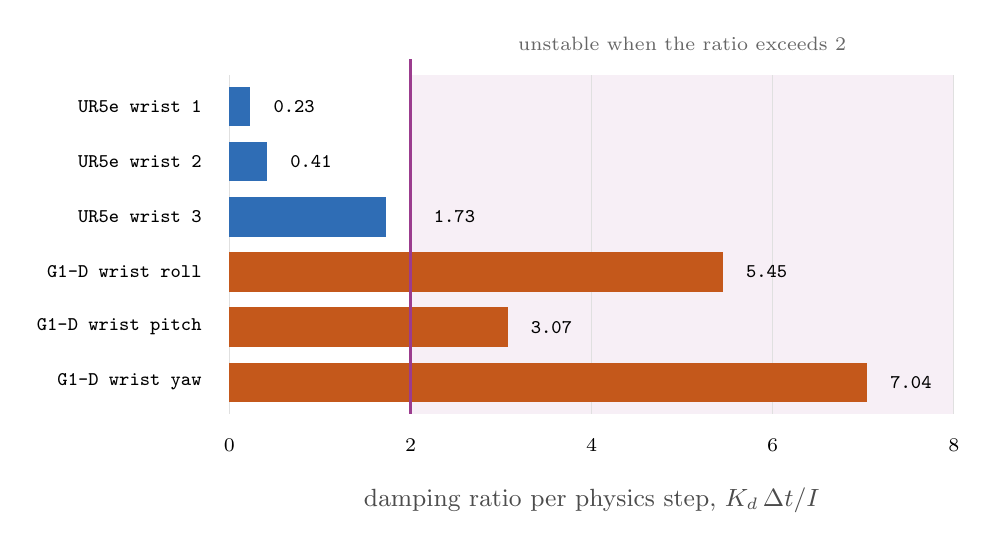
\begin{tikzpicture}[x=1.15mm, y=1mm]
\fill[seriesbad!8] (20,4) rectangle (80,-39);
\foreach \v in {0,2,4,6,8} { \draw[black!12] (\v*10,4) -- (\v*10,-39); \node[font=\scriptsize] at (\v*10,-43) {\v}; }
\node[font=\scriptsize\ttfamily, anchor=east] at (-2,0) {UR5e wrist 1}; \fill[series1] (0,-2.5) rectangle (2.29,2.5); \node[font=\scriptsize\ttfamily, anchor=west] at (3.79,0) {0.23};
\node[font=\scriptsize\ttfamily, anchor=east] at (-2,-7) {UR5e wrist 2}; \fill[series1] (0,-9.5) rectangle (4.15,-4.5); \node[font=\scriptsize\ttfamily, anchor=west] at (5.65,-7) {0.41};
\node[font=\scriptsize\ttfamily, anchor=east] at (-2,-14) {UR5e wrist 3}; \fill[series1] (0,-16.5) rectangle (17.29,-11.5); \node[font=\scriptsize\ttfamily, anchor=west] at (21.50,-14) {1.73};
\node[font=\scriptsize\ttfamily, anchor=east] at (-2,-21) {G1-D wrist roll}; \fill[series2] (0,-23.5) rectangle (54.47,-18.5); \node[font=\scriptsize\ttfamily, anchor=west] at (55.97,-21) {5.45};
\node[font=\scriptsize\ttfamily, anchor=east] at (-2,-28) {G1-D wrist pitch}; \fill[series2] (0,-30.5) rectangle (30.71,-25.5); \node[font=\scriptsize\ttfamily, anchor=west] at (32.21,-28) {3.07};
\node[font=\scriptsize\ttfamily, anchor=east] at (-2,-35) {G1-D wrist yaw}; \fill[series2] (0,-37.5) rectangle (70.41,-32.5); \node[font=\scriptsize\ttfamily, anchor=west] at (71.91,-35) {7.04};
\draw[seriesbad, thick] (20,6) -- (20,-39);
\node[font=\scriptsize, black!60] at (50,8) {unstable when the ratio exceeds 2};
\node[font=\small, black!70] at (40,-50) {damping ratio per physics step, $K_d\,\Delta t / I$};
\end{tikzpicture}
\myfigcaption{fig:stab}{The stability ratio of the UR5e rotational damping applied to each wrist joint. The UR5e stays below 2, with its last joint at 1.73, close to the edge. Every G1-D wrist joint lies above 2, and the wrist yaw sits at 7. The inertias are the diagonal entries of the joint inertia matrix at the default pose, so the bars give a fair estimate rather than an exact bound.}
\end{myfigure}

Translational damping is a different matter. A force at the hand reaches the wrist joints through short lever arms, so the damping that the wrist feels from it is small. The measurements agree. The G1-D with the full UR5e translational damping ran smoothly in every direction, with no sign of chatter.

The actuator joint damping $D$ also escapes the problem. The physics engine solves it as part of the motion rather than applying it as a fixed torque, which keeps it stable at any value. That is why the original author moved the G1-D damping there, and it is also why that location suits the wrist rotation.

%==============================================================================
\section{The Policy Pushes Back}
\label{sec:policy}

So far the action was held at one. A trained policy is under no such restraint. Neither robot clips its actions, and both policies have learned to command far more than one. Table~\ref{tab:actions} shows the size of the actions that three trained policies produced during 160 steps of peg insertion in 32 environments.

\begin{mytable}
\small
\begin{tabularx}{\linewidth}{@{}>{\raggedright\arraybackslash}p{0.19\linewidth}*{4}{>{\raggedleft\arraybackslash}X}@{}}
\toprule
Policy & Translation, 90th pct. & Rotation, 90th pct. & Share above one & Hand speed, 90th and 99th pct. \\
\midrule
UR5e peg, full scale & 2.8 to 4.3 & 6.4 to 19 & 23 to 69 \% & 0.29 and 0.56 m/s \\
G1-D peg, full scale & 1.5 to 4.3 & 2.7 to 9.2 & 18 to 90 \% & 0.30 and 0.94 m/s \\
G1-D peg, quarter scale & 5.0 to 9.8 & 11 to 13 & 34 to 68 \% & 0.26 and 0.55 m/s \\
\bottomrule
\end{tabularx}
\mytabcaption{tab:actions}{Size of the arm actions of three trained policies, per axis, and the resulting hand speed. The action columns give the range over the three axes of each kind.}
\end{mytable}

The last row is the important one. When the action scale was cut to a quarter, the policy simply learned to output larger actions, about two to four times larger than before. The quarter-scale policy now moves its hand at nearly the same speeds as the UR5e policy. Its fastest moments dropped from 0.94 to 0.55 metres per second, but its typical fast motion barely changed. Figure~\ref{fig:stepq} shows the same robot with an action of exactly one.

\begin{myfigure}
\begin{tikzpicture}
\begin{axis}[width=\linewidth, height=0.42\linewidth, xmin=0, xmax=4, ymin=-5, ymax=62, ytick={0,20,40,60},
  xlabel={time (s)}, ylabel={hand displacement along $y$ (mm)}, label style={font=\small}, tick label style={font=\footnotesize},
  grid=major, grid style={black!10}, axis lines*=left, clip mode=individual,
  legend style={font=\footnotesize, draw=none, at={(0.5,-0.24)}, anchor=north, legend columns=1, /tikz/every even column/.append style={column sep=4mm}}]
  \fill[band] (axis cs:1.0,-5) rectangle (axis cs:1.1,62);
  \fill[band] (axis cs:2.0,-5) rectangle (axis cs:3.0,62);
  \node[font=\scriptsize, black!60, anchor=south] at (axis cs:1.05,62) {one step};
  \node[font=\scriptsize, black!60, anchor=south] at (axis cs:2.5,62) {command held for 1 s};
  \addplot[series1, thick] table[x=t, y=ur] {step_q.dat}; \addlegendentry{UR5e, full scale, as trained}
  \addplot[series2, thick] table[x=t, y=g1q] {step_q.dat}; \addlegendentry{G1-D, quarter scale, as trained}
  \addplot[seriesfix, thick] table[x=t, y=fix] {step_q.dat}; \addlegendentry{G1-D, quarter scale, translational damping}
\end{axis}
\end{tikzpicture}
\myfigcaption{fig:stepq}{The quarter-scale G1-D with an action of exactly one. Measured this way it looks calm, at 56 millimetres per second, and translational damping slows it further to 10. The trained policy does not command one, though. It commands five to ten, and the speed grows in proportion.}
\end{myfigure}

This explains why the quarter-scale robot still looked too fast. A policy optimizes for reward, and reaching the peg quickly earns reward. If the controller makes each unit of action smaller, the policy asks for more units. Equation~\eqref{eq:cruise} makes the trade explicit. Any change to the stiffness, the scale or the damping is undone by a matching change in $a$, as long as $a$ is free.

The UR5e policy is no gentler by nature. Its hand reaches 0.56 metres per second in its fastest moments, close to what its 1.57 radian per second joint limit allows. It looks calm partly because its damper keeps every motion smooth and partly because it is a large robot, so the same speed looks slower on it.

%==============================================================================
\section{A Recipe for a Calmer G1-D}
\label{sec:recipe}

Damping is the right instinct, and it belongs in the recipe. It makes the G1-D respond like the UR5e for each unit of action, and it removes the snap at the start and end of each motion. On its own, however, it will not slow the trained robot down, because the policy will learn to push harder. A calmer G1-D needs three changes together, followed by retraining.

\begin{enumerate}
\item \textbf{Add translational damping in the controller.} Set the translational damping ratio to 3, as on the UR5e, and leave the rotational ratio at 0. The measurements show this is stable on the G1-D and that it brings the cruising speed down to the UR5e value of about 43 millimetres per second for each unit of action.
\item \textbf{Damp the wrist rotation in the actuator.} Raise the joint damping of the three wrist joints from 1 to about 2 newton metres per radian per second, and keep it at 1 for the shoulder and elbow. The physics engine handles this damping implicitly, so it stays stable. In the test, the turn about $z$ slowed from 34 to 14 degrees per second, close to the UR5e.
\item \textbf{Bound the action.} Clip the policy output so that the speed formula has a ceiling the policy cannot negotiate away. With a clip at $c$, the fastest the hand can cruise becomes
\begin{equation}
v_{\max} = \frac{K_p\, s\, c}{K_d} \approx 0.047\, c \ \text{m/s}
\end{equation}
at the full scale with the damping of the first step. A clip of 1 gives 47 millimetres per second, which would make a 30 centimetre reach take more than six seconds of a sixteen second episode. A clip of 4 gives about 0.19 metres per second. The clip should be chosen from the speed you want, and the same reasoning sets the rotational ceiling. Section~\ref{sec:oldpolicies} derives a value from a speed that was actually watched.
\end{enumerate}

Table~\ref{tab:recipe} collects the three changes, the setting each one touches and the file that holds it.

\begin{mytable}
\small
\begin{tabularx}{\linewidth}{@{}>{\raggedright\arraybackslash}p{0.14\linewidth}>{\raggedright\arraybackslash}X>{\raggedright\arraybackslash}p{0.15\linewidth}>{\raggedright\arraybackslash}p{0.22\linewidth}@{}}
\toprule
Change & Setting and file & Now & Proposed \\
\midrule
Translational damping & \code{motion\_damping\_ratio} of \code{G1D\_DEX1\_RELATIVE\_OSC} in \path{config/g1d_dex1/actions.py} & 0 on all six axes & 3 on $x$, $y$ and $z$, 0 on the rotations \\
Wrist damping & \code{damping} of the arm actuator in \code{IMPLICIT\_G1D\_DEX1}, file \path{unitree_g1d_dex1/g1d_dex1.py} & 1 on all seven joints & 2 on the three wrist joints, 1 elsewhere, in a second actuator group \\
Action bound & \code{clip\_actions} of \code{G1dDex1\_PPORunnerCfg} in \path{config/g1d_dex1/agents/rsl_rl_cfg.py} & not set & chosen from the target speed, about 7 (Section~\ref{sec:oldpolicies}) \\
\bottomrule
\end{tabularx}
\mytabcaption{tab:recipe}{The proposed changes. None of them is applied in the repository yet.}
\end{mytable}

Two cautions apply. First, the action clip reshapes what the policy can learn, so it calls for a fresh training run rather than a resumed one, and the episode length should be checked against the slower ceiling. Second, the reset-state datasets were recorded with the old controller. They describe poses rather than motions, so they remain valid, but the grasp hold test during recording uses the controller too and may give slightly different yields.

A cheaper check is possible before committing to a full run. Train for a few hundred iterations with each candidate clip, then measure the hand speed percentiles as in Section~\ref{sec:policy}. The 99th percentile is the number that best matches the impression of a robot that moves too fast.

%==============================================================================
\section{Old Policies on the New Controller}
\label{sec:oldpolicies}

Before retraining anything, the two full-scale G1-D policies were run with the controller of Section~\ref{sec:recipe}. The peg policy at iteration 2200 and the cube policy at iteration 1700 were both trained with the old controller. They received the translational damping ratio of 3 and the wrist joint damping of 2, but no action clip, and nothing in the networks changed. The episodes started from the same reset states as the earlier rollouts, so each episode can be compared with its counterpart. Table~\ref{tab:oldsuccess} gives the outcome.

\begin{mytable}
\small
\begin{tabular}{@{}lrr@{}}
\toprule
Policy & Old controller & New controller \\
\midrule
Peg insertion, iteration 2200 & 9 of 10 & 7 of 10 \\
Cube stacking, iteration 1700 & 10 of 10 & 5 of 10 \\
\bottomrule
\end{tabular}
\mytabcaption{tab:oldsuccess}{Successful episodes out of ten for policies trained with the old controller.}
\end{mytable}

The drop is expected. Each policy learned how far the hand travels for a given action, and the new controller moves the hand about five times less for the same action along $y$ and $z$. A policy that expects the hand to arrive in two steps now finds it a fifth of the way there. The peg policy copes better than the cube policy, perhaps because insertion already rewards slow, careful motion near the hole.

The motion looks much calmer, and the numbers agree. Table~\ref{tab:oldspeed} compares the hand speed of the same policies, measured over 160 steps in 32 environments, with and without the new controller.

\begin{mytable}
\small
\begin{tabularx}{\linewidth}{@{}ll*{3}{>{\raggedleft\arraybackslash}X}@{}}
\toprule
Policy & Controller & Hand speed, 50th, 90th, 99th pct. & Turn rate, 90th, 99th pct. & Translation action, 90th pct. \\
\midrule
Peg insertion & old & 0.006, 0.30, 0.94 m/s & 1.18, 3.38 rad/s & 1.5 to 4.3 \\
\rowcolor{band} Peg insertion & new & 0.039, 0.18, 0.32 m/s & 0.78, 1.50 rad/s & 3.0 to 4.6 \\
Cube stacking & old & 0.004, 0.24, 0.86 m/s & 0.87, 3.22 rad/s & 0.8 to 0.9 \\
\rowcolor{band} Cube stacking & new & 0.008, 0.17, 0.32 m/s & 0.72, 1.36 rad/s & 2.8 to 3.1 \\
\bottomrule
\end{tabularx}
\mytabcaption{tab:oldspeed}{Hand speed, turn rate and action size of the same two policies with the old and the new controller.}
\end{mytable}

The fastest moments, the 99th percentile, fell by almost two thirds, from about 0.9 to 0.32 metres per second, and the fastest turns fell by more than half. Those fast moments are what the eye notices, so this is the change that made the robot look calmer.

The last column shows something important. Even without retraining, the policies already push harder. The cube policy roughly tripled its typical action, and the share of its translation actions above one rose from about 9 to about 24 percent. Nothing in the network changed. The policy reacts to what it sees, and a hand that lags behind leaves a larger error in view, so the policy answers with a larger action. This is the closed-loop version of the effect in Section~\ref{sec:policy}, and retraining would only strengthen it.

\paragraph{Keeping this speed after retraining.} A policy retrained on the new controller will learn to use larger actions on purpose, and the speed would creep back up. The action clip of Section~\ref{sec:recipe} prevents that. To keep the speed that was watched here, the cruising ceiling should sit near the fastest moments observed, about 0.32 metres per second. With the damping of Section~\ref{sec:recipe} at full scale, each unit of action buys about 0.047 metres per second of cruising speed, so
\begin{equation}
c \approx \frac{0.32}{0.047} \approx 7 .
\end{equation}
The rotation agrees. With wrist damping of 2, one unit of action turns the hand at about 14 degrees, or 0.24 radians, per second about $z$, and a clip of 7 allows about 1.7 radians per second, close to the 1.4 to 1.5 observed. A clip of 7 therefore preserves the motion that was watched while removing the room to speed up again.

Three limits apply to this estimate. The cruising speeds come from one arm pose, and the forward $x$ direction was much slower there. A clip bounds the steady speed, not the brief surge at the start of a motion, so short peaks a little above the ceiling remain possible. And the success rates above belong to policies that were never trained on this controller, so they say nothing about what a retrained policy will reach. The rollouts are in \path{logs/episode_renders/g1d_peg_newctl_s0}, \path{g1d_peg_newctl_s1} and \path{g1d_cube_newctl}.

%==============================================================================
\section*{How the Numbers Were Measured}

The measurements were taken on 2 November 2026 with the working tree of the \path{feature/forge-omnireset} branch. The step tests come from \path{logs/probe/osc_step.py}, run on the play tasks of both robots with one damping variant and one axis per environment, all starting from the default arm pose with gravity off, as in training. The action statistics come from \path{logs/probe/action_stats.py}, run on UR5e peg iteration 2999, G1-D peg iteration 2200 and G1-D quarter-scale peg iteration 1300, with deterministic actions, and again with the controller of Section~\ref{sec:recipe} for Section~\ref{sec:oldpolicies}. The task-space inertia was computed from the joint inertia matrix of the simulator and the analytical Jacobian of each arm.


\bibliography{references}

\end{document}
